\section{Multiple spines}

\begin{frame}{Multiple spines}
Take multiple spines:
\tikzsetnextfilename{t_two_spines}
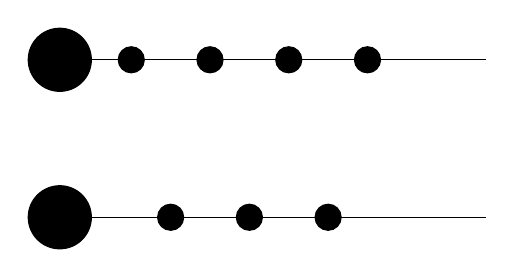
\begin{tikzpicture}

\draw (0, 0) node[left] {$S_2$} -- (5, 0);
\draw (0, 2) node[left] {$S_1$} -- (5, 2);

\tikzstyle{every node}+=[circle,draw,fill]

\node[circle,draw] (o1) at (1, 0) {};
\node[right of=o1] (o2) {};
\node[right of=o2] (o3) {};

\node (u1) at (0.5, 2) {};
\node[right of=u1] (u2) {};
\node[right of=u2] (u3) {};
\node[right of=u3] (u4) {};

\drawedges[bend right]{o1/o2,o1/o3,o2/o3}
\drawedges{o1/u1,o1/u2,o2/u2,o2/u3,o2/u4}
\drawedges[bend left]{u1/u4,u2/u3}

\end{tikzpicture}
%\newProb{\probMul}{Vertex sets~$V_1$, \dots, $V_k$ and
%edge sets $E_0 \subseteq \binom{V_1}{2}$, $E_1 \subseteq V_1\times V_2$,
%\dots, $E_{k-1} \subseteq V_{k-1} \times V_k$, $E_k \subseteq \binom{V_k}{2}$.}{Is there
%a planar drawing of $(V_1 \cup \dotsb \cup V_k, E_0 \cup \dotsb \cup E_k)$ such that
%a vertex in~$V_i$ lies on~$S_i$ for all~$i \in \range{k}$, edges do not cross a spine,
%the edges in~$E_0$ lie completely above~$S_1$ and the edges in~$E_k$ lie completely below~$S_k$?}
Without caps: Solvable in linear time [Jünger et al., 1999].
\end{frame}

\begin{frame}{Level planarity}
Level planarity is an ordering problem:
\begin{figure}[\placement]
\centering

%\resizebox{\textwidth}{!}{
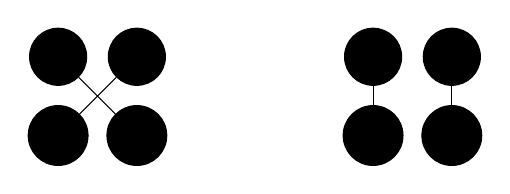
\begin{tikzpicture}

%\tikzstyle{every node}+=[circle,draw]

\node (A1) {$a_1$};
\node[right of=A1] (A2) {$a_2$};
\node[below of=A1] (B2) {$b_2$};
\node[right of=B2] (B1) {$b_1$};
\draw (A1) edge (B1);
\draw (A2) edge (B2);

\begin{scope}[xshift=4cm]
\node (A1) {$a_1$};
\node[right of=A1] (A2) {$a_2$};
\node[below of=A1] (B1) {$b_1$};
\node[right of=B1] (B2) {$b_2$};
\draw (A1) edge (B1);
\draw (A2) edge (B2);
\end{scope}

\end{tikzpicture}
%}
\end{figure}
Forbidden: $a_1 <_i a_2 \land b_2 < b_1$ for $(a_1, b_1), (a_2, b_2) \in E_i$ 
\end{frame}

%\begin{frame}{Observations}
%
%Embeddability only depends on the order of the vertices on the spines:
%\begin{itemize}
%\item Caps come from page embedding
%\item Two edges between TODO
%\end{itemize}
%\end{frame}

\begin{frame}{Mapping to 2-page \probPTree}

\begin{theorem}
A \probMul instance is equivalent to a special 2-page \probPTree instance.
\end{theorem}

\begin{figure}[\placement]
\centering

\resizebox{0.90\textwidth}{!}{
\begin{tikzpicture}

%\draw (0, 0) node[left] {} -- (5, 0);
%\draw (0, -2) node[left] {} -- (5, -2);

%\tikzstyle{every node}+=[circle,draw,fill]

\node (a1) at (1, 0) {$a_1$};
\node[right of=a1] (a2) {$a_2$};
\node[right of=a2] (a3) {$a_3$};

\node (b1) at (0.5, -2) {$b_1$};
\node[right of=b1] (b2) {$b_2$};
\node[right of=b2] (b3) {$b_3$};
\node[right of=b3] (b4) {$b_4$};

\node (c1) at (0.5, -4) {$c_1$};
\node[right of=c1] (c2) {$c_2$};
\node[right of=c2] (c3) {$c_3$};
\node[right of=c3] (c4) {$c_4$};


\drawedges[bend left]{a1/a2,a1/a3,a2/a3}
\drawedges{a1/b1,a1/b2,a2/b2,a2/b3,a2/b4}
\drawedges{c1/b1,c1/b2,c2/b3,c2/b4}
\drawedges[bend right]{c1/c4,c1/c3}

\node[draw=none,fill=none] at (5.5,-2) {{\Huge $\rightsquigarrow$}};

\begin{scope}[xshift=7cm,yshift=-2cm]

%\draw (-1, 0) -- (9, 0);

\node (a1) at (0, 0) {$a_1$};
\node[right of=a1] (a2) {$a_2$};
\node[right of=a2] (a3) {$a_3$};

\node[right of=a3] (b4) {$b_4$};
\node[right of=b4] (b3) {$b_3$};
\node[right of=b3] (b2) {$b_2$};
\node[right of=b2] (b1) {$b_1$};

\node[right of=b1] (c1) {$c_1$};
\node[right of=c1] (c2) {$c_2$};
\node[right of=c2] (c3) {$c_3$};
\node[right of=c3] (c4) {$c_4$};

\drawedges[bend left]{a1/a2,a1/a3,a2/a3}
\drawedges[bend right]{a1/b1,a1/b2,a2/b2,a2/b3,a2/b4}
\drawedges[bend right]{c1/b1,c1/b2,c2/b3,c2/b4}
\drawedges[bend right]{c1/c4,c1/c3}

\end{scope}

\visible<2->{
\node[circle, draw] (r1) at ($ (a2) + (0, 4em) $) {};
\node[circle, draw] (r2) at ($ 0.5*($ (b2) + (b3) $) + (0, 4em)$) {};
\node[circle, draw] (r3) at ($ 0.5*($ (c2) + (c3) $) + (0, 4em)$) {};
\node[circle, draw] (r) at ($ (r2) + (0, 4em) $) {};
\drawedges[ultra thick]{r1/a1,r1/a2,r1/a3,r2/b1,r2/b2,r2/b3,r2/b4,r3/c1,r3/c2,r3/c3,r3/c4,r/r1,r/r2,r/r3}
}

\end{tikzpicture}
}
\end{figure}

\end{frame}